\section{Implementierung}\label{implementierung}

In diesem Kapitel werden die in \ref{zielsetzung} geplanten Verbesserungen an MultiTextCompare durchgeführt und dargestellt. Angegebene Codestücke sind zwecks Lesbarkeit teilweise auf die relevantesten Zeilen gekürzt.

\subsection{Verbesserung des Zeilenmatchings}\label{verbesserungMatching}

Textbasierte Dateien können inhaltlich identisch sein, ohne dass sie exakt gleich aussehen. Sind zwei Dateien inhaltlich identisch aber um eine Zeile verschoben, würden sie von der Software als sehr unterschiedlich bewertet werden. Daher existiert die Matching-Komponente, die sicherstellt dass gleiche oder ähnliche Zeilen erkannt werden, und in der Diff-Anzeige im gleichen Zeilenindex stehen.

Diese Eigenschaft ist daher unerlässlich für den Diff-Prozess innerhalb der Software. Im Kontext der Laufzeit, ist sie aber sehr kostspielig weshalb Maßnahmen notwendig sind, um diese zu senken. Dafür wird hier zunächst die ursprüngliche Funktionsweise in Version 1.0 zusammengefasst dargestellt.

\subsubsection{Optimierung des Matching-Algorithmus}

Das Matching kann in zwei Teilprobleme zerlegt werden. Auf der einen Seite existiert die Matcherkennung, bei der festgelegt wird ob zwei Zeilen überhaupt gematcht werden können. Auf der anderen Seite gibt es noch das Alignment, also die Sicherstellung davon, dass alle Zeilen nach dem Matching korrekt dargestellt werden können. Im Folgenden wird nur auf den ersten Aspekt eingegangen, da dieser die hauptsächliche Funktionalität darstellt.

Um für zwei Dateien A und B alle Matches zu ermitteln, wird zunächst die Datei mit weniger Zeilen als Referenzdatei festgelegt. Dies sei ab jetzt Datei A. In Version 1.0 wurde für jede Zeile von A jede Zeile von B nach einem Match durchsucht. Die Kriterien für ein Match waren dabei, dass sich die Zeilen nach Gleichung (\ref{eq:matchat}) ähnlich genug sind und dass keine der infrage kommenden Zeilen bereits gematcht wurde. Zudem sind Matches \glqq über Kreuz\grqq{} ausgeschlossen. Das heißt, dass die Matchindices für ein potenzielles Match immer größer sein mussten, als die des letzten erfassten Match. Der zugehörige Code ist in Codeabschnitt \ref{code:matchingV1} dargestellt.

\begin{listing}
\begin{minted}
[
frame=lines,
framesep=2mm,
baselinestretch=1.2,
bgcolor=white,
fontsize=\footnotesize,
linenos
]{java}

String ref = "", comp = "";
int lastMatchedIndex = 0;
// Schaue für jede Zeile der linken Datei
for (int i = 0; i < lineCountLeft; i++) {
	reference = leftFile.get(i);
	// ob es in der rechten Datei ein Match gibt
	for (int j = 0; j < lineCountRight; j++) {
		comp = rightFile.get(j);
		if (matches(reference, comp) // falls Zeilen ähnlich genug
				&& j >= lastMatchedIndex // falls Match nicht über Kreuz
				&& notMatchedYet(i, j)) { // falls noch nicht gematcht
			lastMatchedIndex = j;
			// Speichere Match
			matches.add(new IMatchImpl(i, j, reference, comp));
			// Gehe in die nächste Zeile der Referenzdatei
			break;
		}

	}
}
\end{minted}
\caption{Matching in V1.0}
\label{code:matchingV1}
\end{listing}


Besonders ausschlaggebend für die Laufzeit ist dabei die Feststellung der Ähnlichkeit. Für eine Optimierung sollte die Anzahl dieser Feststellungen also, wo möglich, reduziert werden.

Für den Fall, dass in beiden Dateien kein einziges Match existiert, würde jede Zeile von A mit jeder Zeile von B verglichen werden. Dieses Szenario enthält die größtmögliche Anzahl an Vergleichen und stellt daher den worst case dar. Um hier die Laufzeit zu verbessern, wird ein \textit{Lookahead}-Limit eingeführt. Das bedeutet, dass für jede Zeile der Referenzdatei $A_i$ eine maximale Suchreichweite abhängig vom aktuellen Zeilenindex $i$ festgelegt wird.
Als Beispiel würde eine Zeile $A_5$ mit einem Lookahead-Wert von 10 mit jeder Zeile $B_{0...15}$ verglichen werden sofern kein Match für $B_{0...15}$ existiert und Datei B mindestens 15 Zeilen lang ist. Ist Datei B kürzer, so werden alle Zeilen bis zum Dateiende verglichen. 

Auch wenn Matches existieren, kann ein solches Lookehead-Limit Vorteile haben. Für größere Dateien kann es passieren, dass ein Match erst 50-100 Zeilen nach dem letzten gefunden wird. Dies führt dann zu genauso vielen Leerzeilen im Alignment-Prozess, was die Lesbarkeit für den Benutzer beeinträchtigen kann. Da die Eingabedateien vor dem Vergleichen nicht bekannt sind, wird dem Benutzer die Möglichkeit gegeben, den Schwellwert selbst nach Bedarf anzupassen.

Eine weitere Auffäligkeit im Quellcode-Abschnitt \ref{code:matchingV1} ist, dass die Indexvariable j, unabhängig davon ob ein Match gefunden wird oder nicht, immer bei 0 anfängt. Dabei würde es genügen, wenn nach einem Match $M_{i,j}$ der Vergleich erst bei $i = i + 1$ und $j = j + 1$ fortgesetzt werden würde. So müsste auch nicht mehr geprüft werden ob ein Match über Kreuz ist oder ob es bereits ein Match mit den aktuellen Indices gibt. Diese Optimierungen sind im Quellcode \ref{code:lookahead} dargestellt

%TODO: PERFORMANCE UNTERSCHIED BESCHREIBEN%

\begin{listing}[!h]
\begin{minted}
[
frame=lines,
framesep=2mm,
baselinestretch=1.2,
bgcolor=white,
fontsize=\footnotesize,
linenos
]{java}

String ref = "", comp = "";
int lowestPossibleIndex = 0;
// Schaue für jede Zeile der linken Datei
for (int i = 0; i < lineCountLeft; i++) {
	reference = leftFile.get(i);
	int maxSearchIndex = i + LOOKAHEAD + 1;
	if (maxSearchIndex > lineCountRight) {
		maxSearchIndex = lineCountRight;
        }
	// ob es in der rechten Datei ein Match gibt
	for (int j = lowestPossibleIndex; j < maxSearchIndex; j++) {
		comp = rightFile.get(j);
		if (matches(reference, comp)) { // falls Zeilen ähnlich genug
			lowestPossibleIndex = j + 1;
			// Speichere Match
			matches.add(new IMatchImpl(i, j, reference, comp));
			// Gehe in die nächste Zeile der Referenzdatei
			break;
		}
	}
}
\end{minted}
\caption{Aktualisiertes Matching mit Lookahead}
\label{code:lookahead}
\end{listing}

\subsubsection{Verbesserung der Funktionsweise}\label{bestMatch}

Trotz Optimierung gibt es noch einen weiteren Aspekt der verbessert werden kann. Aktuell wird die Suche nach Matches nach dem ersten Match beendet. So entstehen Situationen, bei denen mehrere ähnliche Zeilen nah beieinander existieren und ein Match der ersten möglichen Zeile nicht die beste Option wäre.

\begin{figure}
\centering
\begin{subfigure}{.45\textwidth}
  \begin{minted}{json}
{
  "phones" : [ {
	  "brand": "Apple",
	  "name": "IPhone 12"
  },
  {
      "brand": "Apple",
	  "name": "IPhone 13"
  } ]
}
  \end{minted}
  \caption{Beispiel-JSON 1}
  \label{fig:sub1}
\end{subfigure}
\begin{subfigure}{.45\textwidth}
\begin{minted}[stripnl=false]{json}
{
  "phones" : [ {
	  "brand": "Apple",
	  "name": "IPhone 13"
  } ]
}




\end{minted}
  \caption{Beispiel-JSON 2}
  \label{fig:sub2}
\end{subfigure}
\caption{Zwei ähnliche JSON-Dateien}
\label{fig:bestMatchJSON}
\end{figure}

In Abb. \ref{fig:bestMatchJSON} sind zwei JSON-Dateien abgebildet, bei denen dieses Szenario zutrifft. In der Standardeinstellung würden, bis auf die schließenden Klammern, keine Zeilen der zweiten Datei verschoben werden obwohl in Datei 1 ein identischer Eintrag existiert. Zwar könnte der Wert für $x$ aus Gleichung (\ref{eq:matchat}) auf 1 erhöht werden, allerdings würden dadurch nicht-identische aber ähnliche Zeilen für das Matching ignoriert werden falls die Dateien weitere Einträge hätten.

Die Lösung für dieses Problems wird durch einen \textit{Best-Match} Algorithmus gelöst. Innerhalb des Lookahead-Limits werden alle potenziellen Matches in einer zusätzlichen Liste gesammelt. Mit jedem potenziellen Match wird zusätzlich die \acrshort{llcs} mitgespeichert. Nachdem alle nötigen Zeilen verglichen wurden, wird die Kandidatenliste nach der durch die maximale Länge der verglichenen Strings geteilten LLCS sortiert und das Match verwendet, welches dort den höchsten Wert besitzt. Diese Normierung führt u.\,a. dazu, dass ähnlichere Matches trotz gleicher \acrshort{llcs} bevorzugt werden. Ein Beispiel dafür wäre der Vergleich der Zeilenpaare (\emph{Kunde}, \emph{Kunden}) und (\emph{Kunde}, \emph{Kundennummer}), bei denen die LCS für beide Paare 5 ist, aber die Edit-Distance für das zweite Paar mit 7 deutlich größer ausfällt als die des ersten Paares mit Distanz 1. Dadurch ergäbe sich für Paar 1 ein normierter Ähnlichkeitswert von ca. 0,83 und für Paar 2 ein Wert von nur 0,42, weswegen Paar 1 als Match bevorzugt werden würde. Sollte dieser Wert für zwei potenzielle Matches gleich sein, wird danach entschieden ob eins der Matches direkt auf ein vorangegangenes Match folgt, um möglichst nach verschobenen Blöcken zu suchen. Existiert kein direkter Vorgänger und der Ähnlichkeitswert ist gleich, wird das Match mit geringerem Index verwendet. Das Ergebnis innerhalb der Software ist in Abb. \ref{fig:bestMatchResult} dargestellt. Nun werden alle verfügbaren Zeilen der rechten Datei auch in der linken Datei als existent dargestellt. Das Ergebnis zeigt jedoch auch eine Limitation des Verfahrens. Da es nicht auf die Syntax der unterliegenden Dateiformate eingeht, kann nicht darauf geachtet werden ob ganze Objekte oder Array-Einträge verschoben wurden. Für den hier beschriebenen Fall führt diese Limitation wiederum zu keinen Abzügen in der Genauigkeit bei der Bewertung durch den \emph{Line Compare}-Vergleichsmodus.

\begin{figure}[]
    \centering
    \includegraphics[width=\textwidth]{images/Best Match updated.png}
    \caption{Resultat des Best-Match Verfahrens}
    \label{fig:bestMatchResult}
\end{figure}

\newpage
\subsection{Überarbeitung der Vergleichsalgorithmen}

Das ausschlaggebende Feature der Software ist ihre Ähnlichkeitsmatrix. Diese wurde bereits in der Einleitung kurz erwähnt. Auch die Funktionsweisen der beiden Vergleichsalgorithmen \textit{Line Compare} und \textit{Character Compare} wurden bereits oberflächlich behandelt. Dieses Unterkapitel behandelt nun die Überarbeitung des Modus Line Compare und die Einführung zweier neuer Vergleichsmodi, die sich in ihrer Funktionsweise stark von den bisherigen Algorithmen unterscheiden.

\subsubsection{Zeilenweiser Vergleich regulärer Textdateien}

Line Compare war der erste Vergleichsmodus der Software. Da zum Zeitpunkt der Entwicklung noch keine Matching-Komponente existierte, arbeitete der Vergleichsmodus nicht mehr optimal sobald ähnliche Zeilen leicht verschoben waren. Das Ziel ist nun die Einbettung der Matching-Komponente in den regulären Textvergleich um Dateien, die dem Benutzer in der Diff-Anzeige als ähnlich angezeigt werden würden, auch mit einer höheren Genauigkeit für den Vergleich bewerten zu können.

Alle Vergleiche basieren auf den von der Komponente \emph{FileImporter} erstellten temporären Dateien. Diese sind notwendig um die vom Benutzer ausgewählten Originaldateien bei einer Normierung, also zum Beispiel einer Entfernung aller Leerzeichen, nicht zu verändern. Des Weiteren wurde explizit für den Line Compare Modus ein weiteres Set an temporären Dateien erstellt, bei denen nach jedem Wort ein Zeilenumbruch eingefügt wurde. Als Wort galt eine beliebige Zeichenkette gefolgt von einem Leerzeichen.  

Dieser Prozess sollte eigentlich dazu dienen, um die Genauigkeit des Vergleichs leicht zu verbessern, wobei dies nur für Dateien funktioniert, die ohnehin ähnliche Zeileneinträge in der gleichen Reihenfolge besitzen.

Um die Matching-Komponente in den Vergleich einzubinden, muss zunächst ihre Schnittstelle angepasst werden. Aktuell hat die Matching-Methode \textit{matchLines()} nämlich noch den Rückgabetyp void, denn ihre Erzeugnisse waren bisher immer neue temporäre Dateien im Dateisystem auf die andere Komponenten zugreifen konnten. Um IO-Zugriffe zwecks Laufzeit zu minimieren, erstellt die Methode diese temporären Dateien nicht falls sie für den Vergleich aufgerufen wird. Stattdessen werden die gematchten Zeilen als ein \textit{Object}-Array zurückgegeben. So kann der Rest des Vergleichsalgorithmus unverändert bleiben. Das heißt, dass Zeilen des gleichen Index nach dem in Abschnitt \ref{Levenshtein-Distanz} beschriebenen Verfahren bewertet werden. Sind die beiden zu vergleichenden Dateien nicht gleich lang, wird die kürzere Datei mit Leerzeilen aufgefüllt. Das Ergebnis ist ein zeilenbasierter Vergleichsalgorithmus, der nun verschobene Zeilen erkennen und genauer bewerten kann. Gleichzeitig profitiert er von den in Kapitel \ref{verbesserungMatching} durchgeführen Verbesserungen.

\subsubsection{Vergleich von XML-Dateien}\label{xmlChapter}

\paragraph{Erweiterung der Element-Sortierung}\mbox{}\label{xmlSortierung}

In Version 1.0 besteht bereits die Möglichkeit, die Strukturbäume von XML-Dateien nach ihren Element-Namen und Attribut-Namen zu sortieren. Die Sortierung der Attribute ist insofern eindeutig, als dass ein Attributname pro Element immer einzigartig sein muss. Für Elemente gibt es allerdings keine solche Regel. Elemente, die den gleichen Namen haben und auf der gleichen Ebene innerhalb des Baumgraphen liegen, können als Liste interpretiert werden. 

Vergleichsoperationen wie Line Compare und die Berechnung der Diff würden davon profitieren, wenn XML-Dateien eindeutig sortiert werden könnten, da sie zeilenbasiert operieren. Wenn ähnliche Zeilen in der gleichen Reihenfolge vorliegen, können sie zusätzlich durch das Zeilenmatching erkannt werden. Da weder durch die XML-Spezifikation noch durch die JDOM-API eine Sortierreihenfolge vorgeschrieben wird, wird im Folgenden eine eigene Reihenfolge festgelegt. Diese Priorisierung bezieht sich auf den Vergleich von zwei Elementen:

\newpage
\begin{enumerate}
    \item Elementname
    \item Attributname
    \item Attributwert
    \item Textinhalt
\end{enumerate}

Die Implementierung erfolgt über die Schnittstelle \emph{java.util.Comparator} und das Überschreiben ihrer \textit{compare()}-Methode. Diese gibt einen Integer-Wert zurück mit Hilfe dessen zwei Strings lexikographisch als kleiner, größer oder gleich bewertet werden können. Diese Bewertung wird durch die von JDOM breitgestellte Methode \textit{sortChildren()} ausgewertet, um die Elemente strukturerhaltend zu sortieren.

Sind die Elementnamen identisch, werden die Attribute untersucht. Da Elemente beliebig viele Attribute haben können, werden zunächst nur so viele Attribute verglichen, wie in der kürzesten Attributliste vorhanden sind. Dabei werden erst die Attributnamen verglichen und dann die Werte. Dafür ist vorausgesetzt, dass die Attribute vorher bereits sortiert wurden. Sind die bisher betrachteten Attribute sowohl im Namen als auch im Wert identisch, entscheidet die Anzahl der Attribute. Mehr Attribute werden dabei als größer eingestuft. Bei gleicher Attributzahl werden letztlich noch die Textknoten der Elemente miteinander verglichen. Falls alle dieser Kriterien für die beiden Elemente identisch sind, wird das Verfahren in gleicher Reihenfolge rekursiv für alle Kindknoten der beiden infrage stehenden Elemente durchgeführt, bis ein Unterschied festgestellt wird. Bei Gleichheit der Elemente wird nichts verändert.

\paragraph{Struktureller Vergleich von XML-Dateien}\mbox{}

Im Vorfeld wurden bereits Limitationen der vorhandenen Vergleichsalgorithmen diskutiert. Weder der zeilen- noch der zeichenbasierte Vergleichsansatz kann für Dateien, die einer gewissen Struktur unterliegen zuverlässig für akkurate Ergebnisse sorgen. Aus diesem Grund wird im Folgenden ein Vergleichsalgorithmus entworfen und implementiert, der XML-Dateien auf Basis der Baumstruktur vergleicht.

Verglichen werden sollen dabei die Element-, Attribut-, Text-, CDATA- und Kommentarknoten, wobei letztere optional sind und durch einen Konfigurationsparameter vom Vergleich ausgeschlossen werden können. Ausschlaggebend für den Vergleich sind allerdings die Elementknoten, da jeder der zuvor genannten Knotentypen ein zugehöriges Elternelement hat. Die einzige Ausnahme ist der Wurzelknoten, wobei dieser vom Vergleich ausgenommen ist. Um \emph{false positives} zu vermeiden werden zwei Elemente nur miteinander verglichen werden, wenn ihre Namen identisch sind.

Durch diesen verschiedenen Ansatz, kann das alte Bewertungssystem für die Ähnlichkeit über die LCS oder die Levenshtein-Distanz hier nicht verwendet werden. Stattdessen wird für den strukturellen Vergleich ein Ähnlichkeitsmaß auf Basis der Baumstruktur eingeführt. In Abb. \ref{fig:ähnlichkeitBaum} ist ein Beispielbaum dargestellt, für den die Gewichte der Knoten an der Kante zum Elternelement annotiert sind. Für eine sinnvolle Bewertung wird hierbei davon ausgegangen, dass innerhalb der zu vergleichenden XML-Dateien wichtige Informationen nah am Wurzelelement liegen. Zunächst wird geschaut, wieviele Elemente $n$ innerhalb der ersten Ebene liegen. Jedes dieser Elemente geht mit einem Gewicht von \( \frac{1}{n} \) in den Gesamtwert der Ähnlichkeit ein. Gleichzeitig wirkt dieses Gewicht als ein Budget für dessen Kindelemente. Im Beispiel hat Knoten 2 ein Gewicht von \( \frac{1}{3} \), welches gleichmäßig auf die Kindknoten verteilt wird. Die beiden Kindknoten 5 und 6 haben also im Kontext von Knoten 2 ein Gewicht von \( \frac{1}{2} \). Das Gewicht eines Knotens für die Gesamtähnlichkeit wird berechnet aus dem Produkt aller Kantengewichte $f(V_1,V_2)$ auf dem Weg zwischen der Wurzel und genau diesem Knoten. Dadurch ergibt sich für Knoten 5 bspw. ein Gesamtgewicht von
\[ f(1,2) \cdot f(2,5) = \frac{1}{3} \cdot \frac{1}{2} = \frac{1}{6}\]
\begin{figure}
    \centering
    
\tikzset{eln/.style={midway, font = \Large,inner sep=2pt, outer sep=.30cm}}
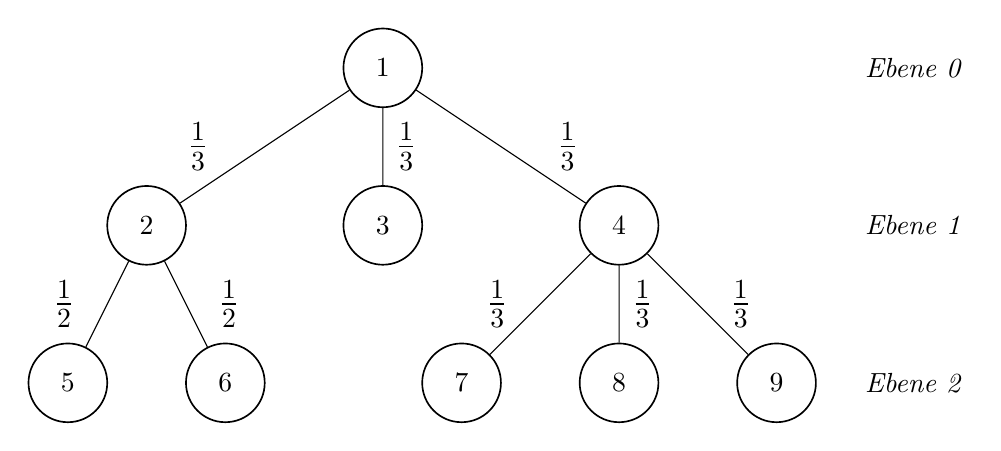
\begin{tikzpicture}[level distance=2cm,
  level 1/.style={sibling distance=3cm},
  level 2/.style={sibling distance=2cm},
  element/.style={circle, draw=black, fill=white, semithick, minimum size=10mm, align=center},
  attribute/.style={ draw=red, fill=white, semithick, minimum size=7mm, align=center},
  textnode/.style={ draw=black, fill=white, semithick, minimum size=7mm, align=center}]
  \node [element](Root){1}
    child {node [element]{2} 
      child {node [element]{5} edge from parent node[left,font = \Large, outer sep=.30cm]{ \( \frac{1}{2} \)} }
      child {node [element]{6} edge from parent node[right,font = \Large, outer sep=.30cm]{ \( \frac{1}{2} \)} }
      edge from parent node[left,font = \Large, outer sep=.60cm]{ \( \frac{1}{3} \)}
    }
    child {node [element]{3} edge from parent node[right,font = \Large, outer sep=0.5mm]{ \( \frac{1}{3} \)}}
    child {node [element]{4}
      child {node [element]{7} edge from parent node[left,font = \Large, outer sep=.30cm]{ \( \frac{1}{3} \)}}
      child {node [element]{8} edge from parent node[right,font = \Large, outer sep=0.5mm]{ \( \frac{1}{3} \)}}
      child {node [element]{9} edge from parent node[right,font = \Large, outer sep=.30cm]{ \( \frac{1}{3} \)}}
      edge from parent node[right,font = \Large, outer sep=.60cm]{ \( \frac{1}{3} \)}
    };
    \begin{scope}[every node/.style={right}]
     \path (Root    -| Root-3-3) ++(5mm,0) node{}  ++(5mm,0) node {\emph{Ebene 0}};
     \path (Root-1  -| Root-3-3) ++(5mm,0) node{}  ++(5mm,0) node{ \emph{Ebene 1}};
     \path (Root-1-1-| Root-3-3) ++(5mm,0) node{}  ++(5mm,0) node {\emph{Ebene 2}};
   \end{scope}
\end{tikzpicture}
    \caption{Gewichtung von Elementknoten für strukturellen Vergleich}
    \label{fig:ähnlichkeitBaum}
\end{figure}

Um diese Gewichte einzusetzen, muss noch definiert werden wodurch zwei Knoten ähnlich sind. Dafür wird bei den Kindknoten der Elemente zwischen textuellem Inhalt, Attributen und Kommentaren unterschieden. Falls Kommentare ignoriert werden sollen oder keine Kommentare präsent sind, sind einzig der Text und die Attribute zu bewerten. Sollten auch keine Attribute existieren, zählt nur der Textinhalt bzw. sollte kein Textinhalt existieren, zählen nur die Attribute. Der Textinhalt schließt reine Textknoten und CDATA-Knoten ein, da JDOM hier auch keine explizite Unterscheidung macht und sie häufig den gleichen Zweck erfüllen. Falls Elemente keinerlei Kindknoten haben, sind sie identisch. Wie Abb. \ref{fig:elementähnlichkeit} zeigt, wird jeder dieser Knoten, sofern er existiert, gleichwertig gewichtet.

\begin{figure}
    \centering
    
\tikzset{eln/.style={midway, font = \Large,inner sep=2pt, outer sep=.30cm}}
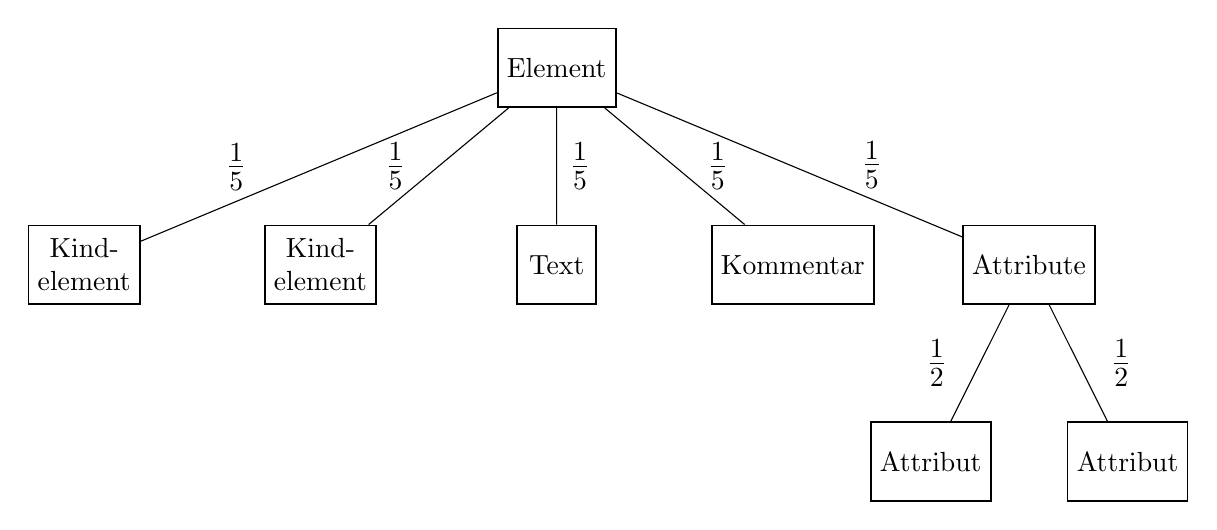
\begin{tikzpicture}[level distance=2.5cm,
  level 1/.style={sibling distance=3cm},
  level 2/.style={sibling distance=2.5cm},
  element/.style={draw=black, fill=white, semithick, minimum size=10mm, align=center},
  attribute/.style={ draw=red, fill=white, semithick, minimum size=7mm, align=center},
  textnode/.style={ draw=black, fill=white, semithick, minimum size=7mm, align=center}]
  \node [element](Root){Element}
    child {node [element]{Kind-\\element}
      edge from parent node[left,font = \Large, outer sep=.80cm]{ \( \frac{1}{5} \)}
    }
    child {node [element]{Kind-\\element}
      edge from parent node[left,font = \Large, outer sep=.30cm]{ \( \frac{1}{5} \)}
    }
    child {node [element]{Text} edge from parent node[right,font = \Large, outer sep=0.5mm]{ \( \frac{1}{5} \)}}
    child {node [element]{Kommentar} edge from parent node[right,font = \Large, outer sep=.30cm]{ \( \frac{1}{5} \)}}
    child {node [element]{Attribute}
      child {node [element]{Attribut} edge from parent node[left,font = \Large, outer sep=.30cm]{ \( \frac{1}{2} \)}}
      child {node [element]{Attribut} edge from parent node[right,font = \Large, outer sep=.30cm]{ \( \frac{1}{2} \)}}
      edge from parent node[right,font = \Large, outer sep=.80cm]{ \( \frac{1}{5} \)}
    };
\end{tikzpicture}
    \caption{Beispielhafte Gewichtung eines Elementinhalts für XML}
    \label{fig:elementähnlichkeit}
\end{figure}

Letztlich muss noch sichergestellt werden, dass das Verfahren symmetrisch ist, also die Reihenfolge der verglichenen Bäume nicht das Ergebnis beeinflusst. Ein Beispiel wäre, wenn der Baum aus Abb. \ref{fig:ähnlichkeitBaum} mit einem Baum verglichen werden würde, der auf Ebene 1 vier Knoten besitzt. In diesem Fall würde die maximale Anzahl an Knoten auf der Ebene entscheidend sein, also läge die maximale Ähnlichkeit der Graphen unabhängig vom Inhalt bei \( \frac{3}{4} \). In jeder Situation bei der unterschiedliche Anzahlen an Einträgen existieren können, wird die gemeinsame Anzahl an gleichen Einträgen durch die maximal verfügbare Anzahl geteilt.  

Implementiert wird dieses Konzept indem zunächst die Wurzelknoten der beiden zu vergleichenden Dateien eingelesen werden, wobei einer der Knoten als Referenzknoten festgelegt wird. Dabei ist nicht wichtig welcher der Knoten die Referenz ist, da in XML das Tauschen von Knoten mit gleichem Elternknoten erlaubt ist. Um diesen Vergleichsmodus anwenden zu können, müssen die jeweiligen XML-Dateien wohlgeformt sein, da ansonsten ein Traversieren der Dokumentbäume nicht möglich ist.

Bei vorliegender Wohlgeformtheit wird zunächst für alle Kindknoten der Referenzwurzel, wie in Quellcode \ref{code:knotenMatching} gezeigt, der aktuelle Knotenname in einer Liste gespeichert. Beim ersten Vorkommen dieses Namens werden alle Elemente mit diesem Namen in einer jeweiligen Liste für Referenzknoten (matchingRef) und Vergleichsknoten (matchingComp) gespeichert. Die Methode \emph{getElementCount()} zählt wie oft ein Elementname in einer Liste vorkommt und sorgt dadurch dafür, dass Elementlisten nicht doppelt eingefügt werden.

\begin{listing}[!h]
\begin{minted}
[
frame=lines,
framesep=2mm,
baselinestretch=1.2,
bgcolor=white,
fontsize=\footnotesize,
linenos
]{java}
        List<Element> matchingRef = new ArrayList<Element>();
        List<Element> matchingComp = new ArrayList<Element>();
        List<Element> refFirstLevelChildren = rootRef.getChildren();
        List<String> refElementNames = new ArrayList<String>();
	for (int i = 0; i < refFirstLevelChildren.size(); i++) {
		Element currentRef = refFirstLevelChildren.get(i);
		String currentRefName = currentRef.getName();
		refElementNames.add(currentRefName);
		if (getElementCount(refElementNames, currentRefName) == 1) {
			matchingRef.addAll(rootRef
					.getChildren(currentRefName));
			matchingComp.addAll(rootComp
					.getChildren(currentRefName));
		}
	}
\end{minted}


\caption{Suche nach gleichnamigen Knoten auf gleicher Ebene}
\label{code:knotenMatching}
\end{listing}\newpage

Da die Matching-Komponente für den strukturellen Vergleich nicht eingesetzt werden kann, muss an dieser Stelle noch ein Mechanismus eingeführt werden um gleiche Listeneinträge zu finden und zu vergleichen. Restliche Listeneinträge können dann noch nach ihrem Index geordnet verglichen werden. Allerdings ist es mit JDOM nicht direkt möglich festzustellen ob zwei Elemente tatsächlich gleich sind ohne alle ihre Kindknoten zu betrachten. Die \emph{equals}()-Methode für die Klasse \emph{Element} prüft nicht auf die inhaltliche Ähnlichkeit sondern ob die Referenz zweier Objekte gleich ist. Dadurch, dass eine rekursive Prüfung aller Kindelemente sehr aufwändig sein kann, wird, wie in Quellcode \ref{code:identischeElemente} gezeigt, mit der Klasse \emph{XMLOutputter} von JDOM gearbeitet. Mit ihr ist es nämlich möglich ein Element als String darzustellen. Da die \emph{equals}()-Methode für Strings \emph{true} zurück gibt sobald die verglichenen Zeichensequenzen identisch sind, kann man auf diese Weise die Gleichheit zweier Objekte feststellen. Um identische Elemente vom rekursiven Vergleich auszuschließen, werden diese durch den Wert \emph{null} ersetzt um sie als bereits bewertet zu kennzeichnen. Nachdem alle verfügbaren Elementknoten miteinander auf Gleichheit untersucht wurden, werden gefundenen null-Werte durch eine Hilfsmethode \emph{clearNullValues}() aus den Listen gestrichen. 

\begin{listing}[!tb]
\begin{minted}
[
frame=lines,
framesep=2mm,
baselinestretch=1.2,
bgcolor=white,
fontsize=\footnotesize,
linenos
]{java}
        for (int i = 0; i < matchingRef.size(); i++) {
		Element currentRef = matchingRef.get(i);
		for (int j = 0; j < matchingComp.size(); j++) {
			Element currentComp = matchingComp.get(j);
			if (currentComp == null) {
			    continue;
			}
			XMLOutputter xmlOut = new XMLOutputter();
			String refString = xmlOut.outputString(currentRef);
			String compString = xmlOut.outputString(currentComp);
			boolean equals = refString.equals(compString);
			if (equals) {
			    similarity.add(currentLevelWeight);
			    matchingRef.set(i, null);
			    matchingComp.set(j, null);
			    break;
			}
		}
	}
	matchingRef = clearNullValues(matchingRef);
	matchingComp = clearNullValues(matchingComp);
\end{minted}
\caption{Suche nach identischen Knoten auf gleicher Ebene}
\label{code:identischeElemente}
\end{listing}

Für die restlichen Elementknoten werden noch die Inhalte verglichen. Der Vergleich von Textknoten, Attributwerten und Kommentaren basiert auf der Levenshtein-Distanz bzw. der Gleichung (\ref{eq:similarityFunc}), da es sich hierbei um reguläre Texte handelt. Bei Attributen werden, wie bei Elementen, nur Attribute mit identischem Namen verglichen. Kommentare werden, falls sie zu mehreren für ein Element existieren, in ihrer originalen Reihenfolge betrachtet. 

Alle aus Quellcode \ref{code:identischeElemente} übrig gebliebenen Knoten in der Liste \emph{matchingRef} bzw. \emph{matchingComp} werden in ihrer bestehenden Reihenfolge rekursiv miteinander verglichen. Falls die Listen unterschiedlich lang sind, werden so viele Elemente verglichen wie sie in der kürzeren Liste vorhanden sind, da die restlichen Knoten ohnehin nicht in beiden Bäumen vorhanden sein können.

\newpage\subsubsection{Vergleich von JSON-Dateien}

\paragraph{Erweiterung der Sortierung}\mbox{}

Anders als bei XML, existiert für JSON die Möglichkeit Elemente nach ihren Namen eindeutig zu sortieren da die Namen bzw. Keys innerhalb einer Ebene eindeutig sind. Innerhalb der Container-Elemente Array und Object existiert ebenfalls eine eindeutige Zuweisung, da Arrays laut JSON-Spezifikation geordnete Listen sind und innerhalb von Objekten auch nach Keys sortiert werden kann.

Falls kein semantischer Kontext für die Reihenfolge der Array-Elemente vorliegt, kann sich eine alternative, konsistente Sortierung, aus den gleichen Gründen wie in \ref{xmlSortierung} beschrieben, lohnen. Auch hier muss zunächst eine Ordnungsreihenfolge festgelegt werden, da Arrays beliebige Elementtypen enthalten können. Inhaltlich werden hierbei nur Knoten des gleichen Typs miteinander verglichen, ansonsten wird folgende Reihenfolge verwendet.

\begin{enumerate}
    \item Valueknoten
    \item Arrayknoten
    \item Objectknoten
\end{enumerate}

Zwei Valueknoten innerhalb des Arrays werden, unabhägig vom Datentyp, über den Text-inhalt ihrer Values als String verglichen.
Für zwei Arrays verläuft der Vergleich zunächst über die Anzahl der Einträge, wobei mehr Einträge als größer bewertet werden. Sind die Arrays gleich groß, entscheidet der Inhalt der Knoten. Es wird so lange über die Arrayknoten iteriert, bis zwei Einträge ungleich sind.
Bei Objekten ist das Verfahren ähnlich wie bei Arrays, nur dass bei gleicher Anzahl an Elementen zunächst die Keys und dann die Values miteinander verglichen werden.

Die in Quellcode \ref{code:jsonArrayRec} gezeigte Implementierung dieser Vergleiche verläuft wie bei XML über einen selbst erstellten Comparator, wobei diesmal für Jackson keine Methode existiert, die den Strukturbaum mit den sortierten Elementen aktualisiert. Stattdessen wird zunächst mittels einer Tiefensuche rekursiv nach Arrays innerhalb des Strukturbaums gesucht. Bei einem Fund, wird das Array sortiert und an die Ursprungsstelle eingefügt. Dafür sorgt die Methode \emph{set}(\emph{int} index, \emph{JsonNode} value) der Klasse \emph{ArrayNode}, die den Knoten am übergebenen Index ersetzt. 

\begin{listing}[!tb]
\begin{minted}[
frame=lines,
framesep=2mm,
baselinestretch=1.2,
bgcolor=white,
fontsize=\footnotesize,
linenos
]{java}
private void sortArraysRecursively(JsonNode currentRoot) {
	if (currentRoot.isArray()) {
	    ArrayList<JsonNode> arrayNodes = new ArrayList<JsonNode>();
	    for (JsonNode node : currentRoot) {
		if (node.isValueNode()) {
		  arrayNodes.add(node);
		} else if (node.isArray()) {
		  sortArraysRecursively(node);
		  arrayNodes.add(node);
		} else if (node.isObject()) {
		  sortArraysRecursively(node);
		  arrayNodes.add(node);
		}
	    }
	    Collections.sort(arrayNodes, new JsonArrayComparator());
	    for (int i = 0; i < arrayNodes.size(); i++) {
	      ((ArrayNode) currentRoot).set(i, arrayNodes.get(i));
	    }
	} else if (currentRoot.isObject()) {
	    for (JsonNode node : currentRoot) {
    	    if (node.isValueNode()) {
    	      //besitzt keine Kindelemente
    	    } else if (node.isArray()) {
    	      sortArraysRecursively(node);
    	    } else if (node.isObject()) {
    	      sortArraysRecursively(node);
    	    }
	    }
	}
}
\end{minted}
\caption{Rekursive Sortierung aller Arrayknoten}
\label{code:jsonArrayRec}
\end{listing}

\newpage\paragraph{Struktureller Vergleich von JSON-Dateien}\mbox{}

Das zuvor vorgestellte Konzept für den strukturellen Vergleich baumbasierter Dateiformate soll nun auch für JSON angepasst und angewendet werden. Auf der einen Seite wird es dadurch vereinfacht, dass es in JSON weniger mögliche Knotentypen gibt. Auf der anderen Seite fällt die Konstante weg, dass jegliche Knotentypen immer einen bestimmten Elternknotentyp, wie im Falle von Elementen bei XML, haben. In JSON können, wie in Abb. \ref{fig:jsonBaum} gezeigt, sowohl Arrays als auch Objekte Einträge eines beliebigen Typs haben, wodurch einige Sonderregeln eingeführt werden müssen. Um einen strukturellen Vergleich für JSON anwenden zu können, müssen auch hier die verglichenen Dateien wohlgeformt sein.

\begin{figure}
    \centering
    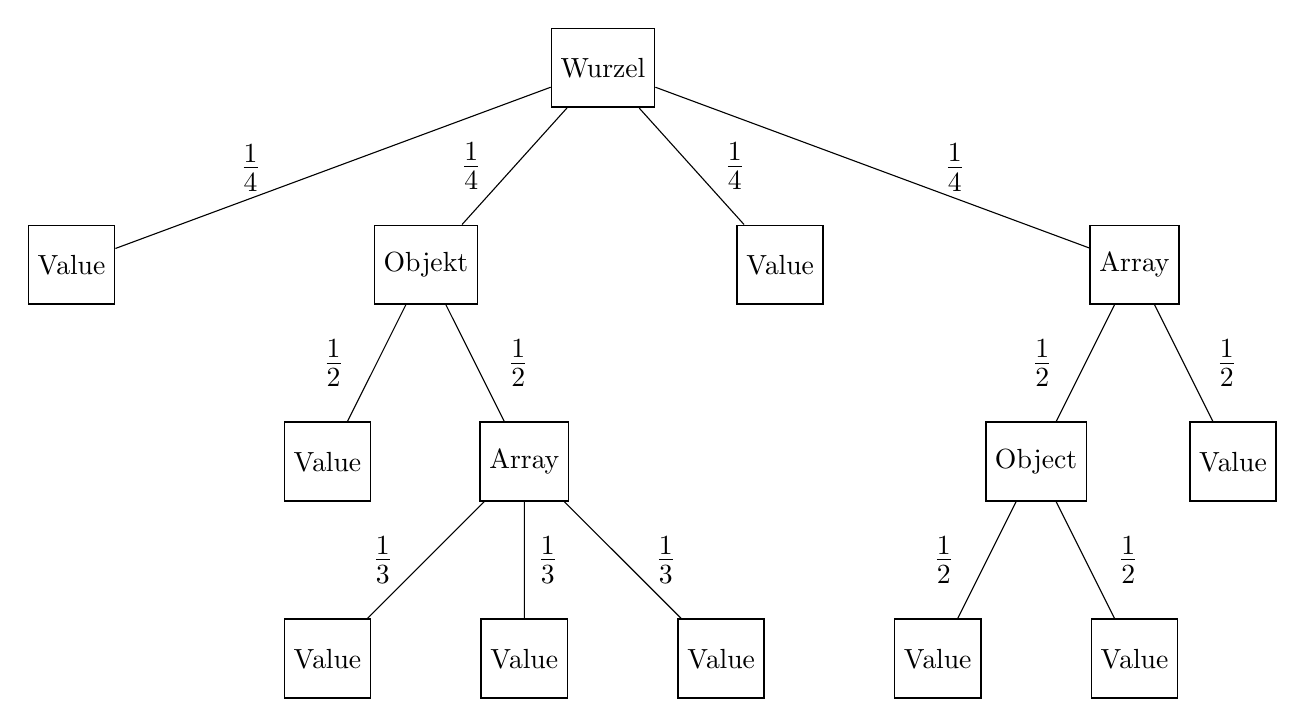
\begin{tikzpicture}[level distance=2.5cm,
  level 1/.style={sibling distance=4.5cm},
  level 2/.style={sibling distance=2.5cm},
  level 3/.style={sibling distance=2.5cm},
  element/.style={draw=black, fill=white, semithick, minimum size=10mm, align=center},
  attribute/.style={ draw=red, fill=white, semithick, minimum size=7mm, align=center},
  textnode/.style={ draw=black, fill=white, semithick, minimum size=7mm, align=center}]
  \node [element](Root){Wurzel}
    child {node [element]{Value}
      edge from parent node[left,font = \Large, outer sep=.80cm]{ \( \frac{1}{4} \)}
    }
    child {node [element]{Objekt}
        child {node [element]{Value} edge from parent node[left,font = \Large, outer sep=.30cm]{ \( \frac{1}{2} \)}}
        child {node [element]{Array}
            child {node [element]{Value} edge from parent node[left,font = \Large, outer sep=.30cm]{ \( \frac{1}{3} \)}}
            child {node [element]{Value} edge from parent node[right,font = \Large, outer sep=0.5mm]{ \( \frac{1}{3} \)}}
            child {node [element]{Value} edge from parent node[right,font = \Large, outer sep=.30cm]{ \( \frac{1}{3} \)}}
        edge from parent node[right,font = \Large, outer sep=.30cm]{ \( \frac{1}{2} \)}}
      edge from parent node[left,font = \Large, outer sep=.30cm]{ \( \frac{1}{4} \)}
    }
    child {node [element]{Value} edge from parent node[right,font = \Large, outer sep=0.3cm]{ \( \frac{1}{4} \)}}
    child {node [element]{Array}
      child {node [element]{Object}
        child {node [element]{Value} edge from parent node[left,font = \Large, outer sep=.30cm]{ \( \frac{1}{2} \)}}
        child {node [element]{Value} edge from parent node[right,font = \Large, outer sep=.30cm]{ \( \frac{1}{2} \)}}
      edge from parent node[left,font = \Large, outer sep=.30cm]{ \( \frac{1}{2} \)}}
      child {node [element]{Value} edge from parent node[right,font = \Large, outer sep=.30cm]{ \( \frac{1}{2} \)}}
      edge from parent node[right,font = \Large, outer sep=.80cm]{ \( \frac{1}{4} \)}
    };
\end{tikzpicture}
    \caption{Beispielbaum für JSON}
    \label{fig:jsonBaum}
\end{figure}

Zunächst werden Knoten über ihre Namen, also ihre Keys gematcht. Sind beide gematchen Knoten vom Typ Value, werden sie nach ihrem Inhalt nach Gleichung (\ref{eq:similarityFunc}) verglichen. Für die Paarung Value- und Arrayknoten wird im Array nach einem Eintrag mit dem Value gesucht. Da das Ziel eine geringe Fehlerquote ist, wird hierbei nur auf exakte Übereinstimmungen geachtet. Andererseits kann hier auch argumentiert werden, dass für eine höchstmögliche Genauigkeit nur Knoten des gleichen Typs verglichen werden sollten. Diese Entscheidung hängt allerdings von der Struktur der Inputdateien ab und ist deshalb nicht eindeutig, weshalb hier auf die Suche im Array gesetzt wird. Value- und Objektknoten werden wiederum nicht miteinander verglichen, da innerhalb des Objekts jedes Element einen eigenen Key hat und es somit keine Möglichkeit gibt, das Value exakt einem Objektelement zuzuordnen. Die einzige Ausnahme wäre, wenn es innerhalb des Objekts ein Element gäbe, welches den gleichen Key hat wie das Elternobjekt. Dieses Element könnte aber auch einen der drei Knotentypen haben weswegen hier auf einen Vergleich verzichtet wird. 

Wenn zwei Arrays miteinander verglichen werden, wird es etwas schwieriger da Arrayelemente weder Keys haben um sie eindeutig zu matchen, noch auf einen bestimmten Elementtyp festgelegt sind. Analog zu den Elementlisten für XML, werden hier zunächst identische Arrayelemente festgestellt und bewertet. Danach folgt die Auswertung der Elementtypen innerhalb der Arrays. Falls Valueknoten innerhalb der Arrays existieren, gelten die gleichen Regeln wie zuvor genannt. Existieren Array-Elemente innerhalb der Arrays, werden diese ebenfalls zunächst durch das Matching ihrer Einträge und dann durch die Fallunterscheidung verglichen. Einträge die nicht gematcht werden konnten, werden in ihrer Reihenfolge verglichen. Zudem werden Arrays und Objekte aufgrund der fehlenden Keys der Arrays nicht miteinander verglichen.

Sollten zwei Objekte innerhalb von Arrays miteinander verglichen oder durch ihre Keys gematcht werden, findet der Vergleich auf Basis der Kindelemente statt. Diese werden über ihre Keys gematcht und je nach Typ mit einer der zuvor genannten Methoden bewertet. 

Die Implementierung basiert im Wesentlichen auf drei Methoden: \emph{compareValues}(), \emph{compareArrays}() und \emph{compareObjects}(). Diese Methoden bekommen als Übergabeparameter die beiden Knoten, die Verglichen werden sollen und liefern ihre Ähnlichkeit zurück. Sie sind so aufgebaut, dass sie sich problemlos gegenseitig aufrufen können, z.\,B. für den Fall dass beim Vergleich von zwei Arrays, zwei Objekteinträge verglichen werden sollen. Zudem funktionieren die beiden Methoden für Arrays und Objekte auch rekursiv, da diese Knotentypen auch Einträge des gleichen Typs beherbergen können.

Das Matching von Arrayeinträgen funktioniert zwar genauso wie das Matching von XML-Elementlisten, die Implementierung weicht aber dadurch ab, dass identische Knoten nicht mehr durch \emph{null} ersetzt werden können, da dies ein gültiger Typ von Valueknoten ist.
Stattdessen wird zu Beginn des Vergleichs ein zufälliger \acrfull{uuid} generiert um einen Wert zu erzeugen, dessen Vorkommen innerhalb einer Datei maximal unwahrscheinlich ist. Um gleiche Arrayeinträge zu finden werden sie mittels der \emph{toString}()-Methode als String dargestellt und über die \emph{equals}()-Methode gematcht. Identische Knoten werden dann im Baum durch einen neuen Arrayknoten ersetzt, welcher lediglich einen Eintrag mit der \acrshort{uuid} beinhaltet. Nach dem Matching werden diese Knoten dann durch die Methode \emph{clearUUIDFields}() entfernt und für den restlichen Vergleich freigegeben. Dafür werden die beiden zu vergleichenden Knoten \emph{fieldValueRef} bzw. \emph{fieldValueComp} mit den veränderten Arrays überschrieben. Dieses Verfahren ist in Quellcode \ref{code:jsonArrayMatching} zu sehen.

\begin{listing}[!t]
\begin{minted}[
frame=lines,
framesep=2mm,
baselinestretch=1.2,
bgcolor=white,
fontsize=\footnotesize,
linenos
]
{java}
        ArrayNode refArray = (ArrayNode) fieldValueRef;
	ArrayNode compArray = (ArrayNode) fieldValueComp;
	for (int i = 0; i < refArray.size(); i++) {
	    String refString = refArray.get(i).toString();
	    for (int j = 0; j < compArray.size(); j++) {
		  String compString = compArray.get(j).toString();
		  if (compString.equals("[\"" + uuid + "\"]")) {
		      continue;
		  }
		  if (refString.equals(compString)) {
		      similarity += currentLevelWeight
				  * calcLevelWeight(fieldValueRef, fieldValueComp);
			  refArray.set(i,objectMapper.createArrayNode()
			 		.add(uuid));
			  compArray.set(j,objectMapper.createArrayNode()
			        .add(uuid));
			  break;
		  }
	    }
	}
	refArray = clearUUIDFields(refArray, uuid);
	compArray = clearUUIDFields(compArray, uuid);
	fieldValueRef = refArray;
	fieldValueComp = compArray;
\end{minted}
\caption{Array-Matching für JSON}
\label{code:jsonArrayMatching}
\end{listing}
%iwas zum matching hier

\newpage
\subsection{Batch-Processing für Vergleiche}
Dem Benutzer ist es möglich, beliebig viele Dateien für den Vergleich miteinander auszuwählen. Da die Software in der Version 1.0 für die Vergleiche single-threaded war, konnte dies je nach Dateimengen- und größen zu langen Laufzeiten führen. Die in \ref{Levenshtein-Distanz} beschriebene Levenshtein-Distanz hat in ihrer Berechnung für zwei Strings $S_1, S_2$ mit der Länge $m$ und $n$ in der verwendeten Implementierung von Apache Commons eine Laufzeit von $\mathcal{O}(m \cdot n)$ \autocite{levenshteinLaufzeit}, was die Laufzeit für lange Zeileneinträge drastisch erhöht.

\begin{equation}
    N = \sum_{k = 2}^{n} k-1 = \sum_{k=1}^{n-1} k = \frac{n ^ 2 -n}{2} \ ,mit \ n\in\mathbb{N}_{\geq2}
    \label{eq:vergleichsanzahl}
\end{equation}

In Gleichung (\ref{eq:vergleichsanzahl}) ist beschrieben, wie viele Vergleiche $N$ für $n$ vom Benutzer ausgewählte Dateien entstehen. Das Minimum an Dateien ist hierbei 2, da es in dem Kontext der Software keinen Mehrwert hat eine Datei mit sich selbst zu vergleichen. Was jedoch auffällt, ist wie stark die Anzahl der zu berechnenden Vergleiche mit der Anzahl der importierten Dateien wächst.

\begin{figure}[!htb]
\centering

\begin{tikzpicture}
\datavisualization [scientific axes, all axes={grid},
    x axis={label=$n$, length=10cm},
    y axis ={label=\begin{turn}{-90}$N$\end{turn}, length=5cm},
    visualize as scatter]
    data {
       x, y
    5, 10
    10,45
    15,105
    20,190
    25,300
    30,435
    35, 595
    40, 780
    45, 990
    50, 1225
    55, 1485
    60, 1770
    65, 2080
    70, 2415
    75, 2775
    80, 3160
    85, 3570
    90, 4005
    95, 4465
    100, 4950
    };

\end{tikzpicture}
\caption{Skalierung der Vergleichsanzahl}
\label{fig:vergleichsskalierung}
\end{figure}

Dies ist für relativ geringe Anzahlen an Dateien in Abb. \ref{fig:vergleichsskalierung} dargestellt. Dadurch entsteht die Frage, wie die Laufzeit der Vergleiche reduziert werden kann, ohne die Genauigkeit der Ergebnisse zu verschlechtern.

Eine Möglichkeit um die Laufzeit drastisch zu verringern, wäre eine Parallelisierung der Vergleiche. So bekäme jeder Prozessorkern (oder jeder Thread bei Mutlithread-Prozessoren) einen Batch (Stapel) an Vergleichen zugewiesen, den er bearbeiten kann. Zusätzlich sollte sicher gestellt werden, dass jeder Thread ungefähr gleich stark belastet wird um die CPU möglichst gleichmäßig auszulasten.

Für die Umsetzung wird zunächst die Java-Klasse \emph{IComparison} aus der \emph{Entity}-Komponente erweitert. Objekte dieser Klasse speichern Referenzen auf die verglichenen Dateien und den Ähnlichkeitswert eines Vergleichs. Dazu kommt nun ein Feld für die ID und ein Feld für das Gewicht des Vergleichs. Die ID ist notwendig, da die Objekte nach ihrem Gewicht auf die verfügbaren Threads verteilt werden und nach dem Vergleich aller Dateien wieder in die ursprünglichen Reihenfolge zusammengefügt werden müssen. Das Gewicht wird hierbei durch die Gesamtzahl der Zeichen dargestellt. 

Zwar beachtet dieses Gewicht nicht, ob die Zeichen gleichmäßig auf die Zeilen verteilt sind, jedoch approximiert es die mittlere Berechnungsdauer. Sollten Zeilen mit besonders vielen Zeichen in den verglichenen Dateien existieren, besteht die Möglichkeit für den Benutzer eine Obergrenze für die Edit-Distance anzugeben, was die Laufzeit in diesem Fall deutlich verringert.

Um die gewichteten Vergleiche nun auf die verfügbaren Threads zu verteilen, werden sie zunächst absteigend nach ihrem Gewicht sortiert. Danach wird mittels der Codezeile
\begin{minted}{java}
Runtime.getRuntime().availableProcessors();
\end{minted}
die Anzahl der Threads und damit die Anzahl der zu befüllenden Batches ermittelt. Um die Vergleiche auf die Batches zu verteilen wird das \emph{Round-Robin}-Verfahren verwendet, bei dem alle Batches nacheinander einen Vergleich zugewiesen bekommen bis alle Vergleiche verteilt sind. 

Um nun jeden Batch auf einem eigenen Thread zu berechnen, wird sobald der Benutzer den Vergleich startet im jeweiligen Event-Handler ein SwingWorker erstellt. Innerhalb dessen \emph{doInBackground()}-Methode wird wiederum ein \emph{ExecutorService} angelegt. Ein ExecutorService liefert Methoden, mit denen Threads und Threadgruppen synchronisiert gestartet bzw. gestoppt werden können \autocite{executorService}. Für das Interface ExecutorService existieren mehrere Implementierungen wobei hier die Implementierung \emph{newFixedThreadPool}(\emph{int} nThreads) verwendet wird. Der Übergabeparameter \emph{nThreads} steht dabei für die Anzahl an Threads, die innerhalb des ExecutorService verwendet werden können. Diese Anzahl wird ebenfalls auf die Anzahl der verfügbaren Prozessorthreads festgesetzt um jedem Thread genau einen Batch zuzuweisen. 

Die \emph{shutdown()}-Funktion des ExecutorServices lässt alle zuvor erstellten Threads zu Ende laufen und baut diese anschließend ab. In der \emph{done()}-Methode des SwingWorkers werden dann alle Batches wieder in eine einzige, nach IDs sortierte, Liste vereinigt und für die Anzeige freigegeben.

\subsection{Verbesserung der UI und der Bedienbarkeit}

Neben der Funktionalität, spielen das Aussehen und die Bedienbarkeit einer Software eine große Rolle. Eine Software sollte möglich intuitiv bedienbar sein und dem Benutzer bei der Bedienung durch Hinweise und Erklärungen Hilfestellung leisten können. 

\subsubsection{Kosmetische Änderungen}
Ob eine Software mit Hilfe von Java Swing erstellt wurde, kann häufig am Aussehen festgestellt werden. Das liegt am von Swing als Standard eingestellten \emph{\acrfull{lnf}}, dem sog. \glqq Metal\grqq{}-Theme. Das \acrshort{lnf} verändert, wie der Name schon sagt, das Aussehen und Verhalten von Swing-Komponenten. Der Vorteil des Metal-\acrshort{lnf}s ist, dass es cross-platform ist und daher unabhängig vom zugrundeliegenden Betriebssystem eingesetzt werden kann. Der Nachteil ist das teils veraltete Aussehen und die stellenweise schwierige Bedienung. Als Beispiel ist in Abb. \ref{fig:metalFileSelection} eine Dateiauswahl mit dem Metal-\acrshort{lnf} dargestellt. 

\begin{figure}
    \centering
    \includegraphics[]{images/metalFileSelection.png}
    \caption{Dateiauswahl unter Metal-\acrshort{lnf}}
    \label{fig:metalFileSelection}
\end{figure}

Als Alternative existieren unter Swing noch weitere, vom Betriebssystem abhängige \acrshort{lnf}s. Diese können mit der Zeile
\begin{minted}{java}
UIManager.setLookAndFeel(UIManager.getSystemLookAndFeelClassName());
\end{minted}
automatisch beim Programmstart geladen und angewandt werden. Zwar ist MultiTextCompare zunächst nur als Windows-Software geplant, allerdings wurde sie bisher immer so entwickelt, dass sie auch auf anderen Betriebssystemen lauffähig ist. Deswegen wird immer das dem Betriebssystem zugehörige \acrshort{lnf} geladen. Die in Abb. \ref{fig:windowsFileSelection} gezeigte Dateiauswahl wirkt dank dem Windows-\acrshort{lnf} nun verständlicher und etwas moderner. Unter Linux würde, sofern es installiert ist, bspw. dann das GTK+ \acrshort{lnf} geladen werden \autocite{lookAndFeel}.

\begin{figure}[!htb]
    \centering
    \includegraphics[scale=0.8]{images/windowsFileSelection.png}
    \caption{Dateiauswahl unter Windows-\acrshort{lnf}}
    \label{fig:windowsFileSelection}
\end{figure}

\newpage\subsubsection{Bedienung der Ähnlichkeitsmatrix}

Eine der Anforderungen ist, dass die Software einfach zu bedienen sein soll, jedoch ist die Auswahl der Dateien zur Anzeige der Diff in Version 1.0 in dieser Hinsicht noch nicht optimal. Ein Klick auf eine Zelle innerhalb der Ähnlichkeitsmatrix öffnete eine Diff-Anzeige für die beiden Dateien in der jeweiligen Zeile bzw. Spalte. Um drei Dateien auszuwählen, musste der Benutzer die Spaltenköpfe der Matrix anklicken, was mehrere Probleme beinhaltet. Zum einen musste für jede Datei einzeln die Ähnlichkeit zu anderen Dateien nachgeschaut werden, da die Matrix nicht automatisch die zugehörigen Zellen der ausgewählen Spaltenköpfe gesondert anzeigt. Zum anderen war es nicht möglich nach dem Fund zweier ähnlicher Dateien nach einer dritten ähnlichen Datei zu suchen ohne die ersten beiden immer wieder auszuwählen. Aus diesen Gründen soll das Auswahlsystem komplett überarbeitet werden.

Zunächst sei grundlegend zu erwähnen, dass die Ähnlichkeitsmatrix technisch gesehen eigentlich keine Matrix ist, da diese nicht als Swing-Komponenten existieren. Stattdessen wird eine JTable verwendet, die als erste Spalte Zellen besitzt, die das Aussehen und Verhalten der Spaltenköpfe aus der JTable imitieren. Dies wird durch eine angepasste Version der Klasse \emph{RowNumberTable} von Rob Carrick umgesetzt \autocite{rowNumTable}. Jegliche Funktionen um Klicks des Benutzers innerhalb der Matrix zu bearbeiten basieren also auf den vorgegebenen Funktionen der Klasse JTable. Das Event-Handling dieser Klicks passiert in einer zusätzlichen Handler-Klasse namens \emph{MouseAdapterMatrix}. Diese erbt von der Swing-nativen Klasse \emph{MouseAdapter} und implementiert die Handler-Methode \emph{mousePressed}(), welche das zu handlende Event als Übergabeparameter erhält. 

Praktischerweise lassen sich aus diesem Event die Zeile und Spalte des Klicks auslesen. Da die RowNumberTable die JTable der Matrix einschließt und kein tatsächlicher Teil der klickbaren Matrix ist, verändern sich auch die Indices nicht. 

Um eine Diff-Anzeige zu öffnen soll nun ein Doppelklick notwendig sein, da ein einzelner Klick einfacher zu Fehlklicks führen kann und diese je nach Dateigröße auch eine Wartezeit nach sich ziehen können. Um einen Doppelklick zu erkennen lässt sich die Methode \emph{getClickCount}() auf dem Eventobjekt ausführen. Um drei Dateien auszuwählen, soll nun ein Zwischenschritt eingeführt werden. Zunächst soll es möglich sein eine Zelle als Referenz festzulegen. Dabei werden alle Zellen, die nicht innerhalb der gleichen Zeile und Spalte oder auf der Hauptdiagonale liegen, ausgegraut und sollen damit nicht klickbar sein. Dies führt dazu, dass jeder mögliche Vergleich übersichtlich dargestellt wird und immer genau drei Dateien ausgewählt werden können. Diese Auswahl geschieht dann mit einem weiteren Klick auf eine der farbigen Zelle und führt nicht dazu, dass die Referenzzelle zurückgesetzt wird. Dafür muss der Renderer der JTable wissen, welche Zelle gerade die Referenzzelle ist.

Für solche Fälle existiert eine zentrale Klasse \emph{Management}, die nach dem Singleton-Entwurfsmuster Objekte für sämtliche Klassen instanziiert, von denen genau eine Instanz existieren soll. Zudem können dort Variablen gespeicht werden, die an verschiedenen Stellen im Code gebraucht werden und ebenfalls nur einmal existieren sollten. Beispiele dafür sind die aktuelle Konfiguration der Software oder die eben erwähnte aktuelle Referenzzelle. Für den sog. \emph{TableCellRenderer} wurde die \emph{prepareRenderer}()-Methode so überschrieben, dass sie prüft ob ein boolsches Flag durch die MouseAdapterMatrix im Management gesetzt wurde und dann entweder die Matrix komplett oder nur die Zellen nach den o.\,g. Kriterien koloriert. Das Resultat ist in Abb. \ref{fig:matrixGrau} zu sehen.

\begin{figure}
    \centering
    \includegraphics[width=\textwidth]{images/Matrix_neu.png}
    \caption{Ausgrauen der Matrix}
    \label{fig:matrixGrau}
\end{figure}


\subsubsection{Konfiguration}

Im Laufe dieser Arbeit wurden bereits diverse konfigurierbare Parameter besprochen. Darunter fällt u.\,a. die Auswahl der Vergleichsmodi, die Funktionsweise des Matchings, Parameter zum Sortieren oder Normieren der Inputdateien. Zwar erhöht eine größere Anzahl an Konfigurationsparametern die Komplexität der Software für Benutzer und Entwickler, zeitgleich liefert sie aber auch die Möglichkeit die allgemeinen Funktion des Textvergleichs für die zu vergleichenden Dateien anzupassen. Schließlich sind die vorgestellten Vergleichsalgorithmen lediglich Approximationen der Ähnlichkeit von Dateien nach bestimmten Kritierien und bilden daher keine objektive Bewertung für alle möglichen Arten von Wissensrepräsentation innerhalb der unterstützten Dateiformate. Falls der Benutzer Dateien vergleichen möchte, die nicht ideal mit den aktuellen Parametern verglichen werden würden, wäre es sinnvoll mehrere Konfigurationsdateien erstellen zu können und diese einfach auszutauschen anstatt immer wieder die aktuelle Konfiguration zurückzusetzen oder zu überschreiben.

MutliTextCompare erstellt, falls noch nicht vorhanden, eine Standardkonfiguration basierend auf Key-Value Paaren für jeden Parameter. Um eine alternative Konfiguration zu verwenden, wird in der Standardkonfiguration ein weiteres Feld für den Pfad der aktuellen Konfigurationsdatei hinterlegt. Ist dieses nicht leer und die Datei existiert, wird diese Konfiguration verwendet, ansonsten wird die Standardkonfiguration verwendet. Der Benutzer hat dadurch die Möglichkeit die aktuelle Konfiguration über die UI zu überschreiben oder als neue Datei unter Angabe des Dateinamens zu erstellen.

\subsubsection{Persistenz von Vergleichen}

Trotz der bisher durchgeführten Optimierungen für die Vergleiche und das Matching, können Vergleiche mit vielen, großen Dateien durchaus noch einige Minuten dauern. Solche langen Wartezeiten können sehr unangenehm sein, besonders wenn die gleichen Vergleichsergebnisse zu einem späteren Zeitpunkt wieder gebraucht werden. Es ist allerdings in Java bspw. durch Serialisierung möglich, bestimmte Programmteile persistent zu speichern. 

Nach Erstellung und Anzeige der Ähnlichkeitsmatrix wird die Diff für Dateien erst berechnet, wenn sie vom Benutzer ausgewählt wurden. Falls vergleichsbezogene Parameter geändert werden, muss die Matrix neu berechnet werden, um diese zu sehen. Das heißt, dass es ausreicht genau den Programmzustand wiederherzustellen, bei dem die Matrix gerade erzeugt wurde. Innerhalb des Codes wird dafür die Liste mit den berechneten Vergleichen der Matrix benötigt. Zusätzlich muss die Map der \emph{FileImporter}-Komponente gespeichert werden, die die erstellten temporären Dateien auf die Originaldateien mappt. Letztlich wird eine geordnete Liste der ausgewählten Dateien  bzw. ihrer Dateipfade mit zugehörigem Index gespeichtert. Zwar könnte diese Liste aus der Map wiederhergestellt werden, allerdings müssten dafür einige Methoden zentralisiert oder publik gemacht werden, was die Abhängigkeiten der Klassen und damit die Komplexität der Code-Base weiter erhöht.

Für die persistente Speicherung über Serialisierung muss sichergestellt werden, dass alle zu speichernden Objekte das Interface \emph{Serializable} implementieren. Dies muss nur für die selbst erstellte Matrix bzw. die Klasse \emph{ICompareImpl} nachgeholt werden. Um die Objekte zu serialisieren wird die native Java Klasse \emph{ObjectOutputStream} verwendet und mit einem \emph{FileOutputStream} in eine Datei geschrieben. Der Dateiname ist vom Benutzer wählbar und besitzt immer die Dateiendung \emph{.mtc}. Damit die Objekte korrekt ein- und ausgelesen werden können, müssen diese in der gleichen Reihenfolge geschrieben und gelesen werden.

Da die Map des FileImporters nur Referenzen auf die Dateien enthält, muss noch sichergestellt werden dass die temporären Dateien eines Vergleichs mitgespeichert werden um die an den Dateien vorgenommenen Normierungen und Sortierungen korrekt anzuzeigen. Dafür wird für jeden gespeicherten Vergleich ein Verzeichnis erstellt, indem sowohl die mtc-Datei mit den gespeicherten Objekten, als auch ein Verzeichnis mit den zugehörigen temporären Dateien vorliegt. Diese temporären Dateien werden dann in das \emph{TempFiles}-Verzeichnis der Software kopiert sobald der jeweilige Vergleich geladen wurde.

\subsubsection{Benutzerfeedback und Logging}\label{logging}

Beim Öffnen von MultiTextCompare erscheint in der unteren Hälfte des Panels ein Log. Dieser dient dazu, dem Benutzer Feedback zu seinen Aktionen zu liefern, bspw. wenn eine Referenzzelle bei der Auswahl von Dateien für die Diff-Anzeige selektiert wird. Zusätzlich werden so Fehler beim Parsen oder interne Fehler während der Laufzeit an den Benutzer weitergegeben. Bisher gab es jedoch keine Unterscheidung nach der Schwere des Fehlers oder der Wichtigkeit der Nachricht, was durch eine interne Logging-Komponente geändert werden soll. Wie bereits im Kapitel zu Architektur in \ref{architektur} gezeigt wurde, funktioniert diese Logging-Komponente außerhalb der eigentlichen 3-Schichten-Architektur. 

Es existiert zwar im Paket \emph{java.util.logging} bereits eine native Logging-Lösung, aber sie ist hier fast schon zu umfangreich und benötige mehr Arbeit um sie in die Code-Base einzupflegen. In der eigenen Logger-Komponenete werden nur 3 Log-Level unterschieden: 
\begin{description}
\item[Info] Beinhaltet das Feedback zur User-Interaktion und Benachrichtigungen über Berechnungen wie den Beginn des Vergleichs und das Ende mit der Berechnungsdauer. Hier handelt es sich um optionale Ausgaben, die besonders dann signifikant sind, wenn eine Berechnung länger dauert oder sich der Benutzer bei der Bedienung der Software noch nicht sicher ist. Diese Ausgaben werden als regulärer Text im Log hinterlegt.

\item[Warning] Bei diesem Level werden Fehler aufgeführt die entweder durch falsche Benutzung der Software auftreten oder durch fehlerhafte Inputdateien. Ein Beispiel für falsche Benutzung wäre z.\,B. der Versuch einen Vergleich persistent zu speichern bevor überhaupt eine Matrix erzeugt wurde. Warnings führen nicht zu Fehlverhalten und werden mit roter Schrift auf gelbem Hintergrund im Log angezeigt.

\item[Error] Errors sind schwerwiegende Fehler, die dazu führen dass das Programm nicht ordnungsgemäß funktionieren kann. Der wahrscheinlichste Fehler auf diesem Level ist eine \emph{FileNotFoundException}, die geworfen wird falls Dateien unerwartet gelöscht, verschoben oder umbenannt wurden. Diese Fehler werden im Log mit rotem Hintergrund und weißer Schrift angezeigt.
\end{description}

Zusätzlich zur Anzeige im Log werden diese Ausgaben auch persistent in Logdateien gespeichert. Um riesige Logdateien und damit einen Verlust der Übersicht zu vermeiden, werden die Logs nach Datum getrennt. Für jede Logausgabe wird dafür geprüft ob eine aktuelle Logdatei existiert, ansonsten wird eine neue Datei erstellt. Zwar werden alle Logausgaben unabhängig vom Level in die Logdateien geschrieben, dem Benutzer ist es aber möglich einzelne Level für die Anzeige im Log ein- und auszuschalten.
